% *************************************************************************
\chapter[Computational Enzyme Engineering: Activity Screening by Quantum Chemical Methods.]
{Computational Enzyme Engineering: Activity Screening by Quantum Chemical Methods.\label{ch1}}
\chapauth{Martin R. Hediger$^{a}$
\chapaff{$^{a}$Z\"urich\\
m---@---.ch}}
% *************************************************************************


% *************************************************************************
% *************************************************************************
\section{Abstract}\label{sec:abstract}
Main messages:
\begin{itemize}
\item QM Screening of CALB and BCX
\item Screening 317 single and 111 double mutants with av. 29 h per barrier and 1 CPU per interpolation point
\item Correct mechanisms using PM6
\item Barriers in agreement (calc. 18.5, exp. 17.0 kcal/mol)
\item 15/22 correctly predicted (using many approximations and not full model)
\item No bias, more active double mutants identified
\item largely automated
\item For CALB lowest barriers close to WT, BCX lowest barriers lower than WT
\end{itemize}
% *************************************************************************


% *************************************************************************
% *************************************************************************
\section{Motivation}\label{sec:mot}
Let us imagine two companies $a$ and $b$.
Both companies use very similar technical equipment to carry out the biotechnological process $\ce{X}$ $\xrightarrow{Biocatalyst}$ $\ce{Y}$ using two different versions of a biocatalyst.
Company $a$ uses an enzyme with a rate constant $k_{a} = 1000s^{-1}$ while company $b$ uses an enzyme with $k_{b} = 2000s^{-1}$.
Letting all other things be equal, the process of company $b$ will therefore only require half the time to produce one Mole of product compared to the time required for company $a$.
Company $b$ therefore can save energy required to keep the reaction volume at a certain temperature.
The need for efficient catalysts arises from such an outline and the commercial implications of these considerations are immediate.\footnote{In this work, we use the terms \textit{enzme} and \textit{bio-}/\textit{catalyst} interchangeably.}\\
Increasing the performance of enzymes however is still far from trivial and forms a growing body of research.
What is clear though is that the development of such catalysts is costly, in terms of manpower, material and energy -- if carried out in the laboratory.
A number of companies have in fact formed around this demand: Novozymes (DK), Genzyme (US) or DSM (NL) to name but a few\cite{meyer2013use, kirk2002industrial, beilen2002enzyme, schmid2002use}.\\
Laboratory costs can however be saved to a large part if the development is carried out \textit{in silico}.
The proof that computational results are as reliable as experimental results has been provided not too long ago\cite{claeyssens2006high}.
The foundation for successful application of computational enzyme engineering has thus been laid out.
It is therefore natural to ask: Why hasn't this become more important yet?
Why are there not more job openings at pharmaceutical and biotechnology companies looking for computational enzyme engineers?
The field, after all, did receive the Nobel price in Chemistry in 2013.
As a side note, computational modeling of aero- and fluid dynamics, semiconductor properties, pharmaconkinetics/pharmacodynamics or civil engineering is well beyond the point of having to justify itself as of strategic relevance.\\
More important questions asked and answered in this review:
\begin{itemize}
\item Is it possible to screen for mutant activity using quantum chemical methods?
\item Which quantum chemical model can reproduce the accepted mechanism?
\item What are the time requirements depending on the model size?
\item How should the program be configured?
\item What modeling procedure/sequence is needed? Which tools are useful?
\end{itemize}
By giving an overview and some details in this article, I hope to, at least in part, answer the above questions.\\
\textcolor{red}{[ARE THE QUESTIONS ANSWERED?]}
% *************************************************************************


% *************************************************************************
\section{Introduction}\label{sec:intro}
In this review, we aim to provide an introduction into the topic of modeling of enzyme catalysis for people from both within or from outside the field, with emphasis on aspects of activity screening and some emphasis on commercial applicability.
We outline the latest achievements, methods in use and required developments to further establish computational enzyme engineering and screening also in commercial practice.\\
While the process engineering team in company $a$ from above is working on improving reaction conditions, consider the enzyme engineer required to engineer the currently used catalyst to match (and possibly outperform) the activity of the catalyst used by company $b$.
Following the hypothesis that the function of an enzyme depends on its structure, in order to change the function, some kind of change to the structure has to be introduced and this in general requires the introduction of one or more mutations of amino acids in the primary structure of the enzyme.
However, as is well known in the community, it is almost impossible to predict, how a mutated variant of an enzyme will behave[\textcolor{red}{REFS?}, Bornscheuer?].
Will it at all be possible to express it and will it even fold and if so, will it be more or less active and specific relative to the wild type?
Are its pH properties still the same and is it of similar temperature stability?
Even the most reasonably suggested mutations (except for elimination of the catalytic residues) will not allow to predict \textit{qualitatively} with confidence if the mutated enzyme will be more or less active.
Therefore it appears as if the only reasonable strategy were to carry out systematic screening studies.\footnote{By \textit{screening} we mean the construction of a large library of mutants which are inspected and compared for a specific property like activity.}
As was pointed out initially, such studies are expensive in the laboratory and therefore an alternative is to carry them out on the computer.
The aim of such initial computational screening is not to provide high-accuracy kinetic data but much rather to provide a reliable, qualitative activity estimate of a preferably large mutant library.
It is important to note that while the initial computational screening might be of limited accuracy, its major value is the provision of a systematically developed library of mutants.
Based on the screening, promising candidates can then be pipelined into a more demanding computational method for further characterization.

\noindent\textcolor{red}{[Physical property of interest:]}\\
The method has to be adapted to the physical property of interest\\
- Thermal and structural integrity\\
- pH dependent activity\cite{ludwiczek2013strategies}\\
- Active site hydration\\
- Binding, \textit{c.f.} drug design where the target protein is constant\\
- Catalysis: \textit{C.f.} biofuel production or synthesis applications where the substrate is mostly non-variable.

\noindent\textcolor{red}{[Different modeling objectives:]}\\
1) One Enzyme -- Multiple Substrates:
These tasks are usually addressed by docking approaches and studies involving millions of substrates have been published\cite{zhou2010high}.\\
2) Multiple Enzymes -- One Substrate:
The approaches to this task, as it appears, are much less established.
Why is that?
A number of factors can be of influence among which are that modeling of different variants of an enzyme will also mean to differentiate between multiple (possibly coupled) protonation states which is non-trivial.
Furthermore, modeling of reactivity always involves modeling of a transition state, which is non-trivial and for which there is no standard fail safe approach.

\noindent\textcolor{red}{[Application context:]}\\
- Academic: screening can assist in generation of new hypothesis about structure/function relationships\\
- Commercial: commercial application is restricted by time-to-delivery of predictions, accuracy/reliability, screening spectrum and convenience of use.
Notefully, in a commercial context, accuracy can be of less value than reliable qualitative prediction of relative activities.

\noindent\textcolor{red}{[Review structure and audience:]}\\
This review is written for a more general audience.
For specialized details, the reader is referred to the primary literature.
Since molecular modeling of enzymes has been reviewed extensively over the recent years, we do not attempt to provide all fundamentals of the subject.
Instead, we focus on screening aspects of computational enzyme engineering.
The intention is to provide an accessible introduction into the field of quantum chemical modeling of enzymatic reactions, highlight advantages of using quantum chemistry and also point out situations where special care needs to be taken.\\
By 2014, quantum chemical methods have been in use to study enzymatic reactions for around three decades.
What is new however is that quantum chemical methods can now be used also in \textit{in silico} screening assays of enzymatic activity and this is also part of the focus of this review.
% *************************************************************************


% *************************************************************************
% *************************************************************************
\section{Methods}\label{sec:methods}
\subsection{Modeling Approaches}\label{sec:modeling}
In all molecular studies, it should be the physical property of interest that guides the selection of the appropriate computational method and not the other way around.
At the most fundamental level, computational descriptions of a molecular system is done by (parametric) \textit{force fields} or \textit{ab initio} electronic structure methods.\footnote{\textit{Molecular mechanics} or \textit{classical mechanics} are other expressions for force field methods.}
Force field methods are useful in studying structural behaviors of enzymes over a significant time period (up to nanoseconds) and can provide details about rearrangement of loop motives.
The description of chemical reactivity however requires the description of the electronic structure of the system (molecular mechanics models do not allow the description of bond formation and braking processes).\\
Another categorization can be made among the different modeling approaches among which these days one can name cluster models (kinetic discrimination of mechnisms, transition state testing), hybrid quantum mechanical/molecular mechanical methods (high-accuracy barrier calculations) and full enzyme structure methods (mutant screening studies).
Each of these in turn are differently suited to model different properties.\\
\textbf{Full enzyme structure methods -- General outline of screening method.}
The presented activity screening method would fall under the last category of the above mentioned.
We have have used this method in two studies where new functionality has been introduced into an enzyme active site using quantum chemical methods\cite{10.1371/journal.pone.0049849,hediger2013silico,hediger2013computational}.\\
In both studies, the basic procedure consists of preparing structures for the enzyme substrate complex (``ES'') and the first intermediate (CALB: ``TI''\footnote{Tetrahedral intermediate}, BCX: ``GE''\footnote{\label{foot:ge}Glycosyl enzyme}) and calculating the reaction barrier between these two pairs of structures, respectively.
The reaction barrier is calculated by interpolating between the ES$_\text{CALB}$ and TI or ES$_\text{BCX}$ GE structures, \textit{i.e.} by preparing a set of 10 intermediate structures which approximate the structure of the system along the reaction coordinate.\footnote{In the literature, the terms \textit{interpolation}, \textit{linear transit scan}, \textit{reaction coordinate calculation} or \textit{adiabatic mapping} are frequently used to indicate the same kind of procedure}.
By evaluating the energies for each interpolation frame for the two reactions ES$_\text{CALB}\rightarrow$TI or ES$_\text{BCX}\rightarrow$GE, it becomes possible to obtain an approximate potential energy surface of the reaction, Fig. \ref{fig:calb_reaction}.
The quality of the results of this approach are strongly dependent on how careful the modeling of each of these structures is carried out.
A frequent reason for meaningless results is significant structural rearrangement during the geometry optimization, requiring to interpolate between very different conformations of the two stationary points on each side of the reaction barrier.\\
Finally, the activities of different variants of an enzyme are ordered by comparing the activation energy required for the rate determining step of the overall reaction -- low activation energies correspond to high anticipated activity of the variant.
Implicitly this assumes high substrate concentration such that $k_\text{cat}$ becomes rate limiting, a reasonable assumption under industrial conditions.\\
\textbf{Requirements.}
The most basic requirements are that a structure representing a bound intermediate along the reaction pathway is available.
Alternatively, a homology model could be used.
Furthermore, ideally the mechanism for the rate determining step is established in the literature.
In case no generally accepted mechanism is reported, a preceeding study could analyse kinetically competing mechanism alternatives.\\
\textcolor{red}{\textbf{[Aspects of model size and modeling.]}}
It is frequently observed that specific pairs of mutants can not be accommodated together because of the size of the side chains.
In order to facilitate the approach, these variants are discarded from the screen.
Furthermore, side chain orientations can be oriented in various ways and are defaulted using some approach (local, empirical function based optimization in PyMOL).
At the least, this removes ambiguity in the modeling step.
Ionization states of side chains greatly complicate the screening and the best approach most likely is to consider different ionization states only at a later stage of the assay.\\
\textcolor{red}{\textbf{[Interpolation/Linear transit/Adiabatic mapping.]}}
\begin{figure}[htbp] 
\centering
\begin{minipage}{0.43\linewidth}
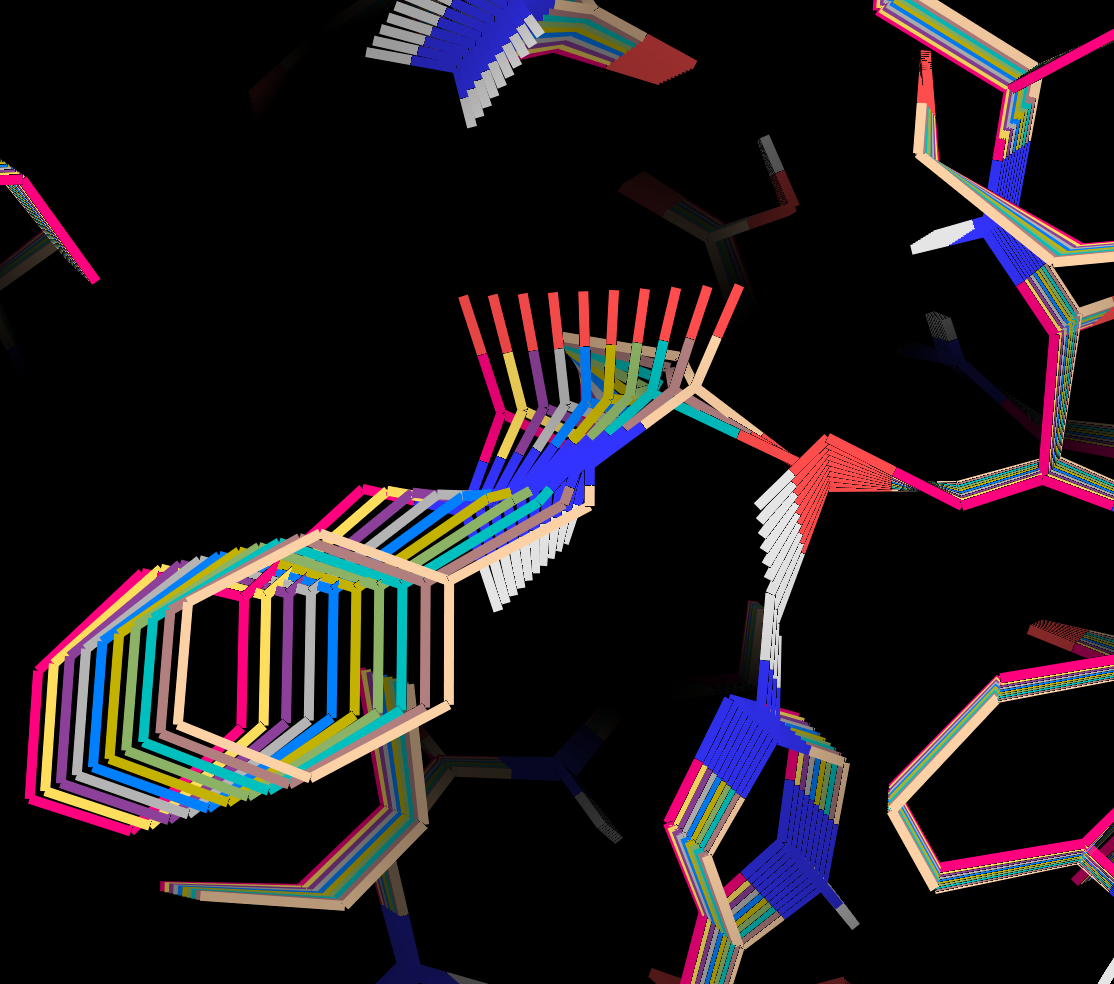
\includegraphics[width=0.90\linewidth]{wt-ini.png}
\end{minipage}
\begin{minipage}{0.55\linewidth}
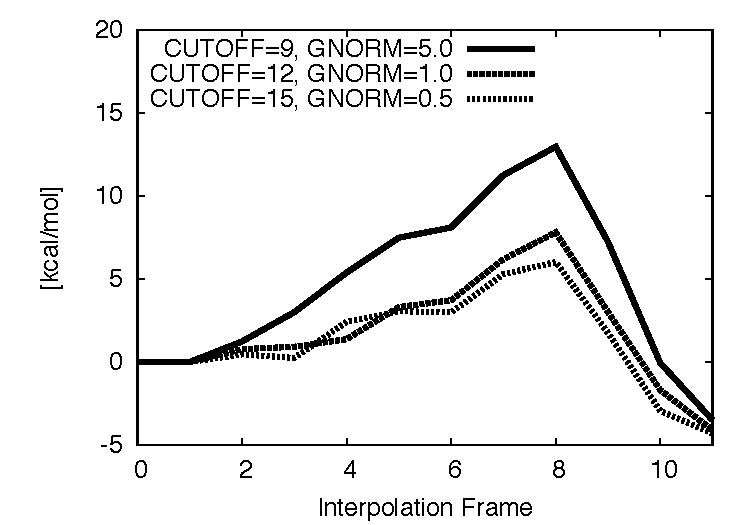
\includegraphics[width=1.00\linewidth]{calb-conv.pdf}
\end{minipage}
\caption{
Intermediate structures along reaction coordinate of CALB reaction.
}
\label{fig:calb_reaction}
\end{figure}



\subsection{\textcolor{red}{Quantum Chemical Calculation Engines}}\label{sec:quantum_chemical_methods}
A number of issues arise in the development of the modeling method.
The method needs to consider the trade-off between accuracy and efficiency, it should be easily set up and allow scale up from a selected few to a large, systematic library of variants.
These criteria encompass not only the calculation engine, but also to the molecular modeling software used in the preparation of the molecular models.
An initial survey revealed that semi-empirical quantum chemical methods meet the requirements of the method.
They are readily available in a number of programs (GAMESS, MOPAC and others), they are very efficient and test calculations show that they (not all) reproduce the generally accepted mechanism of the catalytic triad.\\
It is essential to note that \textit{every method has it's chemistry}.
The results of one quantum chemical method need to be verified, ideally against high-level standard reference methods.
If a method can reproduce the canonical mechanism then there is a good chance that at least qualitatively reliable conclusions can be made using this method.
\begin{itemize}
\item AM1/RM1/PM3/PM6/PM7/MOZYME
\item DFT/B3LYP/Dispersion corrections/M06/...
\item Modeling procedures: Define constraints- how does it affect the calculation (examples in literature?)
\item Explain available software: GAMESS, MOPAC
\item Explain parameters of PM6: MOZYME, gradient convergence and NDDO cutoff
\end{itemize}
\textcolor{red}{[Assessment of semi-empirical methods.]}
Reliability of the quantum chemical method in the studies presented in this review are established by comparing various geometrical parameters (\textit{i.e.} transition-state bond lengths) which allows to identify if a method agrees with the generally accepted mechanism.
Further criteria are then required computational effort and amenability to data analysis and programming.\\

\subsection{Calculation and Modeling Software}\label{sec:software}
Various engines are implemented in different calculation software.
Methods on paper are of limited use if they can not be applied, therefore also available modeling software is a very important factor.\\
Modeling software is available, PyMOL, Schr\"odinger, Chem?? (Walter Thiel, commercially) but everything is still very much custom work (especially the data analysis, programs output format is like from last century), this is probably the major reason preventing the use of QM as standard method in industry.
Compare docking and MD methods have software which is designed towards user friendlyness and has become established in industry.
GTKDynamo is an exceptionally good example for what it should look like, unfortunately only small community.\\
Many studies claim that ``\textit{future developments are directed at further automating the presented approach}''.
Obviously these remarks are directed at making the method industrially applicable by avoiding the requirement to carry out complicated setup and configuration steps\cite{rathore2013advances}.
In reality, such future developments, to the great unfortune of the whole field, are rarely realized -- speculation on the reasons is beyond the scope of this article.
Nevertheless, almost no publication fails to mention the potential applications in drug design.
Computational considerations are only rarely taken into account but greatly help at putting the whole approach into perspective\cite{buch2011complete}.
% *************************************************************************


% *************************************************************************
% *************************************************************************
\section{Activity Screening Applications}\label{sec:apps}
\subsection{Overview}\label{sec:overview}
Independent of the method, a screening assay should be
\begin{itemize}
\item Fast
\item easy to setup
\item qualitative accuracy
\end{itemize}
Practical applicability of QM based enzyme screening has a couple of problems:
\begin{itemize}
\item The structures of the enzyme in the relevant state of the reaction need to be available, ie. an enzyme-substrate complex (ES) and a transition state (TS) analog (usually an inhibited species)
\item If the mechanism is not established, the reaction can usually follow various pathways -- these would need to be checked in order to find a best guess at the rate determining step
\item Identification of the transition state is difficult and depends intimatly on the structure, optimizing two structures differing by 0.1 \AA in a particular bond length can result in identification or not identification of the TS
\item \textcolor{red}{Focus on catalysis, assume binding is similar over mutant range\cite{ludwiczek2013strategies}- $K_\text{M}$s are similar for mutants}
\end{itemize}

% *****************************************************************
\clearpage
\subsection{Engineering {\textit{Candida antarctica} Lipase B}}
\textbf{Relevance and Summary.}
Using CALB as a test case, we develop an efficient modeling protocol, verify the calculations with experimental results and show how quantum chemical methods can be used for enzyme activity screening\cite{10.1371/journal.pone.0049849, hediger2013silico}.
The reaction studied is the hydrolysis of $N$-benzyl-2-chloroacetamide.
CALB has been highly characterized over the years such that its structure, physical properties and expression systems are well documented\cite{uppenberg1994sequence, uppenberg1995crystallographic}.
The enzyme is a highly established catalyst with applications in organic synthesis, formulation technology\cite{gayot2003modification} and in kinetic resolution of racemic mixtures\cite{gotor2006candida, naik2010lipases, chaput2012contribution}.
Furthermore, since the enzyme is known for its reactive promiscuity\cite{bornscheuer2004catalytic, CBIC:CBIC200800318}, it provides an ideal development platform for applications for which existing biocatalysts are of restricted efficiency.
One such application is the hydrolysis of amide bond containing lipophilic compounds.
While in principle amide bonds can be cleaved by proteases or peptidases, these enzymes are found to be less active towards hydrophobic substrates such as amide containing lipids\cite{nakagawa2007engineering}.
Therefore, engineering CALB activity towards ${\text{CO}-\text{NH}}$ bond containing hydrophobic substrates would greatly expand its applicability and provide a new tool to the toolbox of chemical biotechnology.\\
\textbf{Structure and Mechanism.}
Briefly, the active site in CALB consists of a catalytic triad (S105, D189 and H224) and an associated oxyanion hole.
The mechanism is understood to follow the generally accepted mechanism of serine protease active sites\cite{hedstrom2002serine}, Fig. \ref{fig:calb-mechanism}.
\begin{figure}[htbp] 
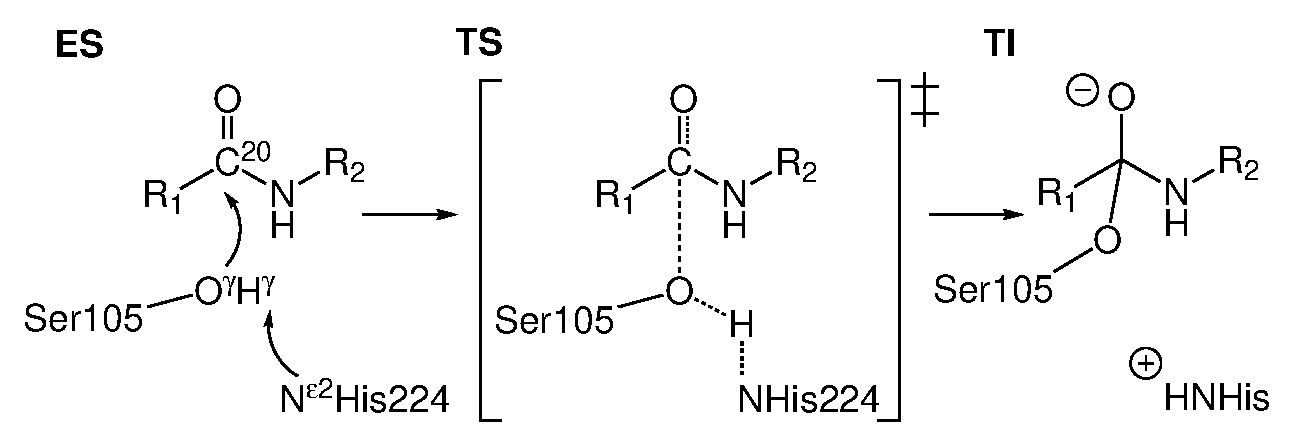
\includegraphics[width=0.98\linewidth]{calb-mechanism.eps}
\caption{
Reaction scheme for the formation of the tetrahedral intermediate in CALB.
In this work, R$_1$: -CH$_2$-Cl, R$_2$: -CH$_2$-C$_5$H$_6$\cite{hediger2013silico}.
}
\label{fig:calb-mechanism}
\end{figure}
The rate determining step is believed to be the nucleophilic attack by O$^\gamma$ of S105 on the carbonyl carbon C$^{20}$ of the substrate.\\
\textbf{Scale up, Experimental Verification and Calibration.}
After establishing a proof-of-concept of the screening approach using a limited set of three mutants\cite{10.1371/journal.pone.0049849}, the method was scaled up to screen a set of 386 mutants of the CALB active site\cite{hediger2013silico}.
This set consisted of single- to eight-fold mutants and the activity of 22 mutants of the set was measured experimentally.\\
The method was calibrated in terms of qualitative prediction rate, \textit{i.e.} how likely can the method predict if a mutant will have higher or lower activity than the wild type.
This calibration requires to note a couple of issues which are discussed in the following.
In the experiments, the activity relative to the WT, in principle, ranges from zero to infinity.
In the calculations on the other hand, the activity of a mutant is determined by the difference between the mutant reaction barrier and the wild type barrier.
Even for a very active mutant, the reaction barrier is not expected to be zero and so in this approach, since lower barriers are related to higher activities, the amount by which a mutant can be more active than the wild type is in principle limited.
Conversely, since the reaction barrier of a mutant can in principle be arbitrarily high, the amount by which a mutant could be less active than the wild type might be infinite.
A direct quantitative relationship between reaction barrier differences and relative experimental activities is therefore not very meaningful, the value of a computational screening study in a production environment is to indicate which mutants should be considered for further study, and not so much to quantify their activity.
Instead, only qualitative relative activities (higher or lower than WT) are determined, both for the experimental and calculated results, and used for the calibration of the predictivity.\\
To cluster the results into increased/decreased activities it is therefore necessary to decide above/below which activity a mutant is considered being part of either the higher-activity or lower-activity clusters.
Considering the relatively narrow spread of experimental activities\footnote{The experimental improvement factors range from 0 to roughly 11 times wild type activity.}, mutants with $\geq1.2$ times the wild type activity are considered improving while mutants with $<0.8$ times the wild type activity are considered degrading (mutants inbetween are considered as neither improving nor degrading)\cite{hediger2013silico}.
The computational results are clustered in a similar way.
A cutoff value for the calculated reaction barriers is introduced \textit{below} which the mutant is considered improving and above which the mutant is considered degrading.
Subsequently, out of the mutants predicted to have higher activity, a set containg as many mutants as can be further characterized is selected and suggested for further study, either computationally or experimentally.
It is found that at a specific cutoff value (12.5 kcal/mol), the method qualitatively predicts activity of 15 out of 22 mutants correctly, Fig. \ref{fig:diag-predictivity}.
\begin{figure}[htbp] 
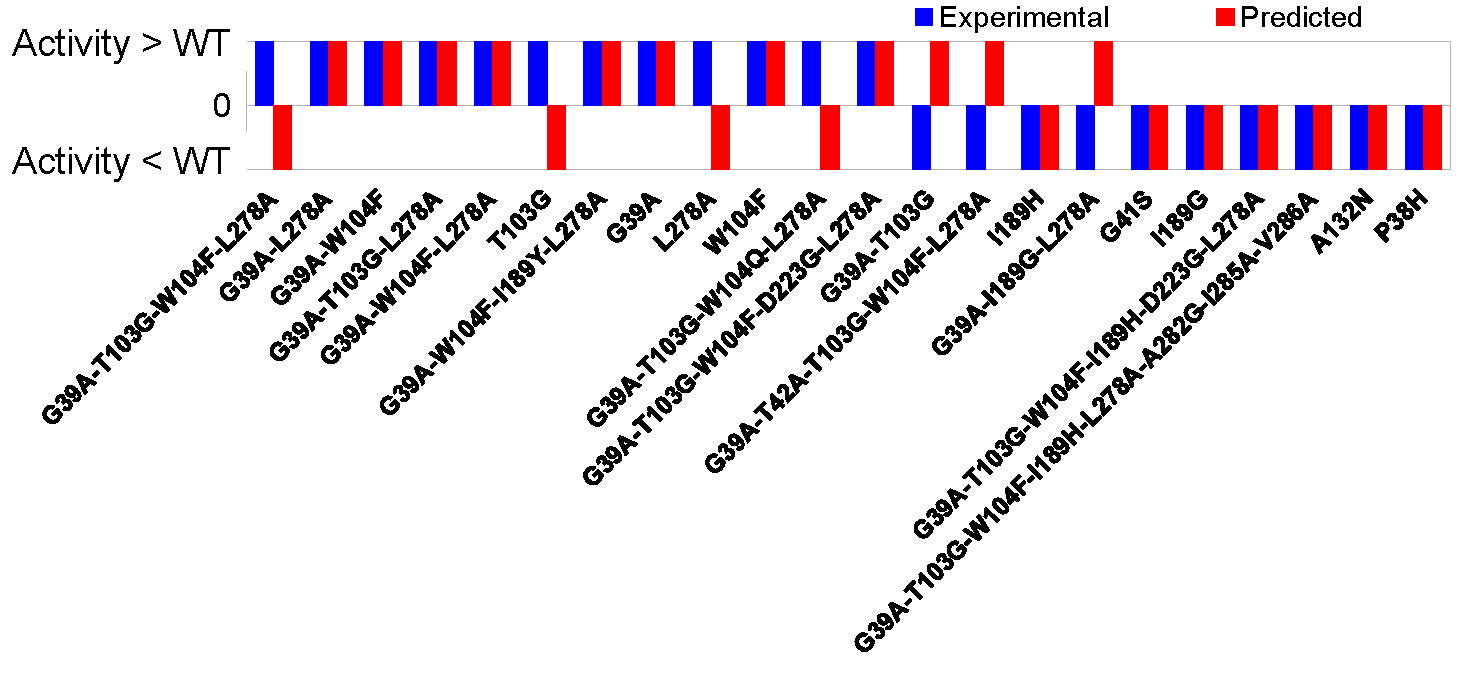
\includegraphics[width=1.00\linewidth]{diag-predictivity-truncated.pdf}
\caption{
Agreement between predicted and experimental qualitative activity relative to wild type\cite{hediger2013silico}.
}
\label{fig:diag-predictivity}
\end{figure}
Noteworthy, mutants with both higher as well as lower activity are correctly predicted.
Importantly, the advantage of clustering the mutants in this way is not apparent maximum agreement with the experimental data in the first place, but much rather to provide a lower limit for the predictivity under the given set of approximations.
It needs to be kept in mind that in such a computational enzyme activity assay, it is unlikely to have calibration data available since it is performed \textit{before} wet-lab experiments are carried out.
We find this approach furthermore justified since at the initial outset of a screening study, the focus is mostly on narrowing down possible candidates from a large library, \textit{i.e.} the focus is on obtaining qualitative conclusions rather than quantitative results\cite{agresti2010ultrahigh}.\\
\textbf{Screening Results and Discussion of Mutants.}
In the set of 386 screened mutants, we identified only three mutants with a barrier lower than the wild type (a double, a triple and a four-fold mutant).
Analysis of the screening results was further focused on two residues: W104 and I189.
These are selected because mutations of these positions can provide more space for the substrate which is hypothesized to lead to increased activity, Fig. \ref{fig:calb-views}.
\begin{figure}[htbp] 
%\centering
%\begin{minipage}{0.42\linewidth}
\textbf{A}
%\end{minipage}
%\begin{minipage}{0.42\linewidth}
%\textbf{B}
%\end{minipage}
%\begin{minipage}{0.49\linewidth}
%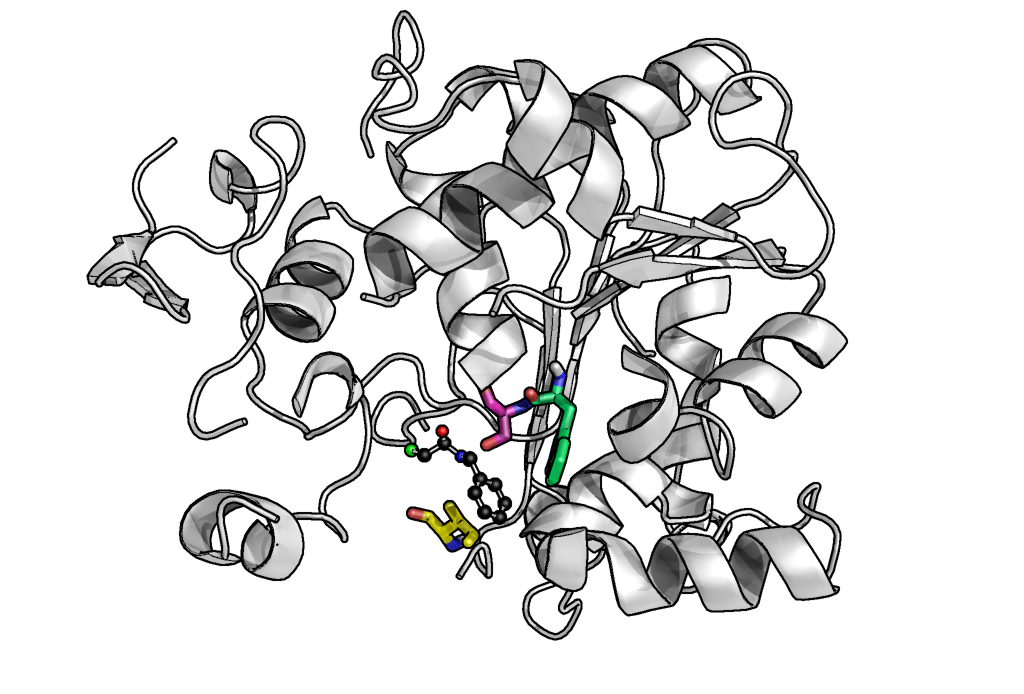
\includegraphics[width=0.95\linewidth]{calb-total-view.png}
%\end{minipage}
%\begin{minipage}{0.49\linewidth}
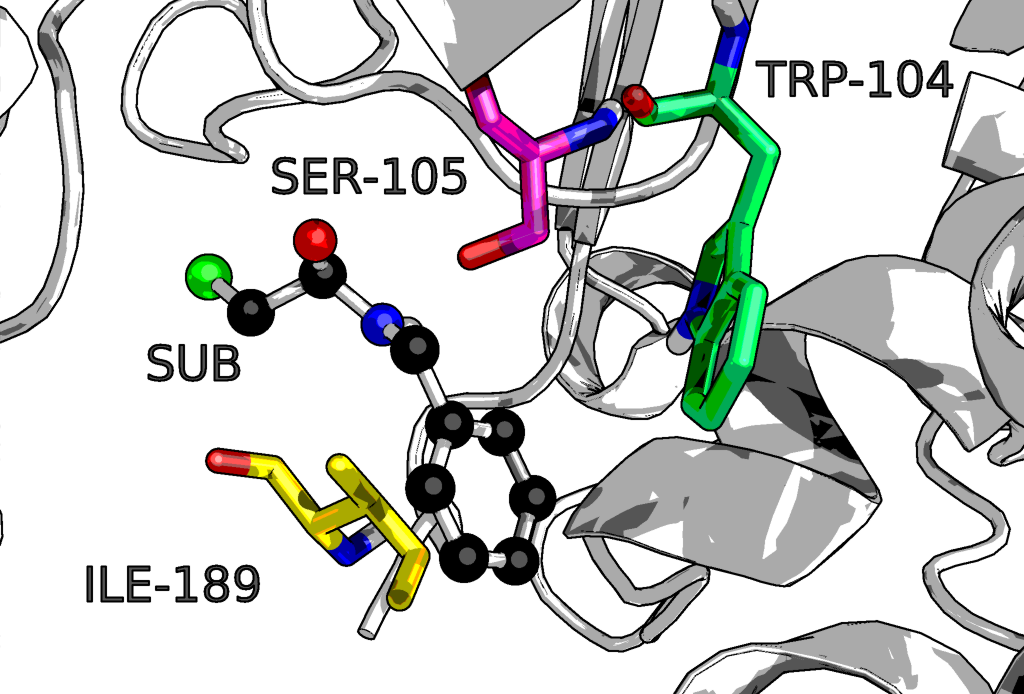
\includegraphics[width=0.95\linewidth]{calb-active-site.png}
%\end{minipage}
\caption{
%\textbf{A}: CALB total view, active site visible in the lower part of the panel.
%\textbf{B}: Active site, some residues omitted for clarity.
CALB active site, some residues omitted for clarity.
SUB labels the substrate.
}
\label{fig:calb-views}
\end{figure}
As seen, W104 and I189 are in direct proximity to the substrate.
From the single mutant data, it is found that the mutants W104Q or W104Y have barriers just around the cutoff value of 12.5 kcal/mol.
However, when in combination with other mutations, such as G39A-W104F-A141Q-I189A (8.3 kcal/mol) or G39A-T103G-W104Y-A141N (9.8 kcal/mol), these mutations are among the most active ones found and it is clear that arriving at such combinations by purely rational considerations is virtually impossible.\\
Analysis of mutations of I189, Fig. \ref{fig:i189g} provides additional intersting insight.
\begin{figure}[htbp] 
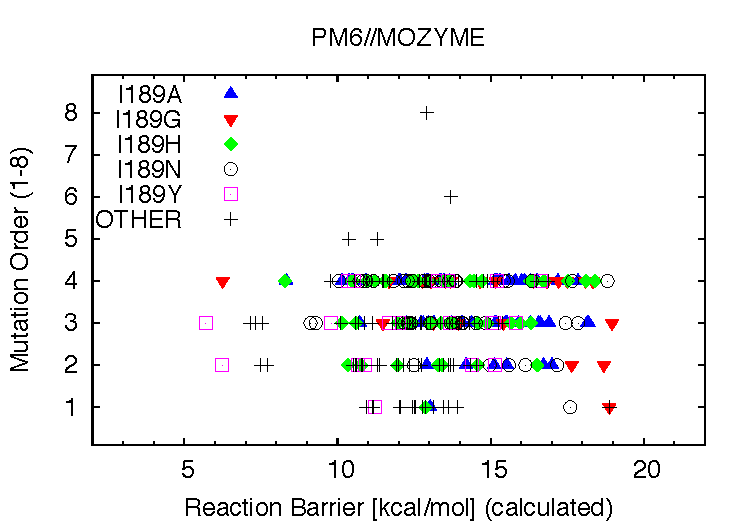
\includegraphics[width=0.95\linewidth]{011-diag_eval_scre_setL-i189.pdf}
\caption{
I189G screening.
}
\label{fig:i189g}
\end{figure}
Five different mutations are screened but the analysis is focused on I189G.
As a single mutant, I189G is found to be completely unproductive (18.9 kcal/mol), in a double mutant the barrier is reduced in one case to around 17.5 kcal/mol and in G39A-A141Q-I189G-L278A, the I189G mutation is among the top three mutants found (6.3 kcal/mol).
Conversely, the mutant G39A-A141Q-L278A has a moderately low barrier (10.9 kcal/mol).
These results emphasize the fact that the activity modulating effect of specific point mutations behaves strongly non-linearly and should be kept in mind when considering which mutations to include in further studies.
Put differently, these findings illustrate that it is difficult to predict the activity of combination mutants based on single mutant data alone.
Since, apparently, single mutant data is not sufficient to predict combination mutant activity, screening a wide library of mutants should form an essential initial part of any enzyme engineering project.
Furthermore, it is immediately clear that computational activity screening, thus, can provide major advantage in cost and material use reduction to the overall enzyme engineering efforts.\\
\textbf{Outlook.} A number of points remained unaddressed in this study.
Among these is the fact that not the complete enzyme structure was used in the calculations, instead only amino acids within 8$\AA$ of the substrate have been included in the model.
The backbone sequence is therefore interrupted, introducing ambiguity in how to orient hydrogen atoms used to complete the valences at the interruption points.
Secondly, the set of positions screened was directed by prior knowledge, instead of an unbias systematic screening and lastly, it remained to be shown that the presented approach was also useful for mechanistically different reactions in different enzymes.
%
% Weak points of the study to be addressed in BCX project:
%\begin{itemize}
%\item Selection of model ambiguous/not full structure
%\item Not systematically screening all mutants
%\item No other protein system/enzymatic reaction tested
%\item Binding effects not considered
%\item Large rearrangements can not be modeled
%\item Semi-empirical methods might not be adequate for metals
%\item Subsequent steps of reaction not modeled (eg. product leaving of active site)
%\item Different ionization states of residues
%\item From a modeling point of view it's a disadvantage not to include the full structure in the calculation because there is ambiguity on how to model the backbone termini
%\end{itemize}
% -----------------------------------------------------------------

\clearpage
\subsection{Engineering \textit{Bacillus circulans} xylanase}
The xylanase of \textit{Bacillus circulans} is applied in paper production\cite{bajpai1999application, buchert1994application}.
Fields related to degradation of plant materials are \textit{e.g.} biofuel production.\\
In order to address the points summarized above and to show general applicability of the approach outlined for CALB, the xylanase of \textit{Bacillus circulans} (BCX) is engineered to be catalytically active towards an artifical substrate ($ortho$-nitrophenol-$\beta$-xylobioside), Fig. \ref{fig:substrate}.
\begin{figure}[htbp] 
\centering
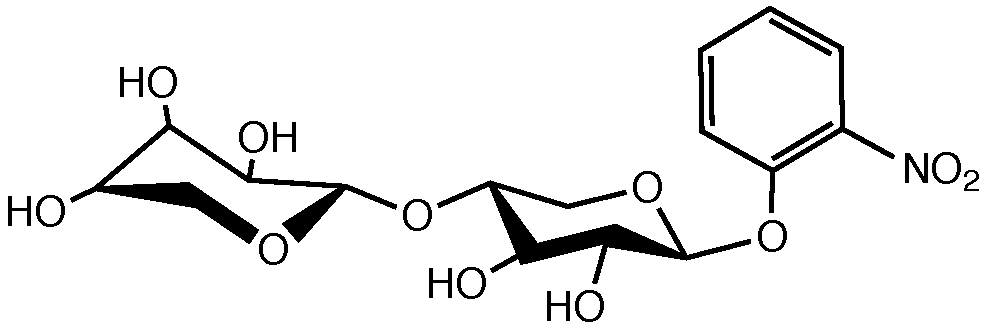
\includegraphics[width=0.85\linewidth]{substrate.pdf}
\caption{
$ortho$-nitrophenol-$\beta$-xylobioside substrate used in BCX study consisting of two xylose units and ONP.
}
\label{fig:substrate}
\end{figure}
In this study, the mechanism was taken from the literature as reported previously\cite{joshi2000hydrogen,joshi2001dissecting}.
In the following, we outline the work reported in the study and illustrate the sequence of simulation and modeling steps.\\
\textbf{WT reaction barrier modeling.}
In a first step, the wild-type (WT) reference reaction barrier is established.
This is a crucial step because all subsequent conclusions about mutants are depending on how good the WT reaction barrier is estimated.
As was done for CALB, only the rate determining step is modeled, Fig. \ref{fig:bcx_mechanism}.
\begin{figure}[htbp] 
\centering
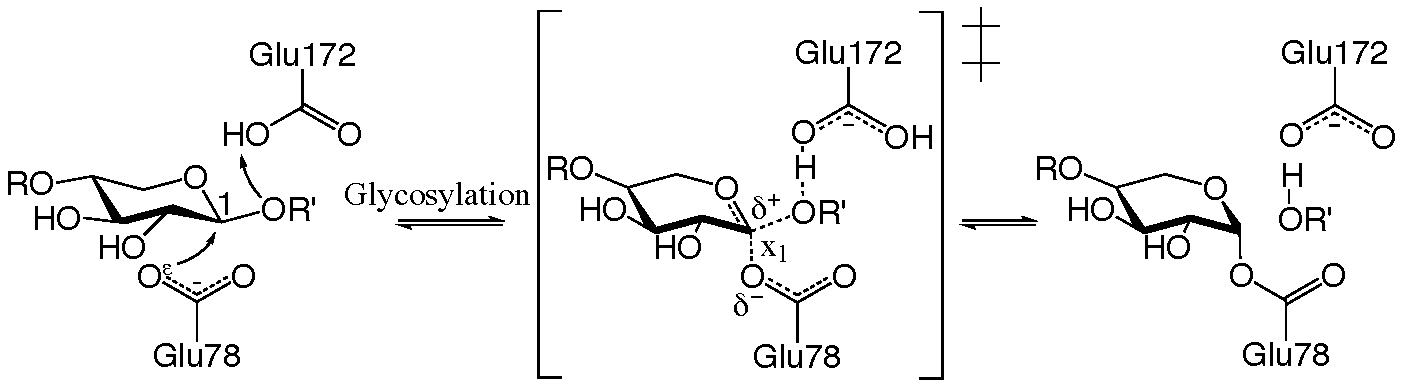
\includegraphics[width=1.0\linewidth]{mechanism.pdf}
\caption{
Rate determining step in conventional glycosylation. $x_1$: constrained reaction coordinate; $R$: xylose; 
$R'$: \textit{ortho}-nitrophenol (ONP).
C$_1$ indicating nucleophilic carbon of first xylose unit\cite{hediger2013computational}.
}
\label{fig:bcx_mechanism}
\end{figure}
As outlined in the methods section, the reaction barrier is mapped out by fixing the reaction coordinate ($x_1$ in Fig. \ref{fig:bcx_mechanism}) at discrete, decrementing values while optimizing the rest of the protein structure.
Since the reaction consists of two concerted events (nucleophilic attack by E78 and proton transfer from E172 to ONP), in principle a two-dimensional potential energy surface could be mapped out to determine the reaction barrier.
However, since proton transfer is associated with a rearrangement of the electronic structure, this reaction coordinate is left unconstrained and is handled solely by the quantum chemical method, \textit{i.e.} the proton is free to transfer from or remain on E172.
Forcing the quantum chemical model to do something it would not if left unconstrained most likely results in an increased reaction barrier and therefore it is advisable to keep the number of constraints as low as possible.\\
A PDB structure comprising a covalently linked inhibitor is available (1BVV) and is used as a starting point for the modeling procedure because it gives a very clear indication of how the substrate is located in the active site.
As shown in Fig. 2 in Hediger \textit{et al.} (2013b), two possible modeling pathways were worked out.
In the first one, the ES complex is prepared from the GE structure \textit{before} the GE structure is optimized (see footnote \ref{foot:ge}).
Alternatively, the GE structure is optimized first and then used as a template for the ES structure.
Within this alternative approach, the preparation of the ES structure then just requires minor modifications of substrate conformation before the structure is optimized.\\
Because in this second approach the ES structure very closely resembles the optimized GE structure, it is possible to concentrate the optimization of the ES structure only on the active site, while the remote part of the enzyme remains fixed at the optimized geometry of the GE structure.
This results in very large gains in computational efficiency, which depend on the layer of residues being optimized around the active site.\footnote{The structural constraints are parameters to the calculation program and are prepared programmatically using a PYMOL script. The way the parameters are submitted to the calculation may vary depending on the software used for calculations.}
Fixing, \textit{i.e.} not reoptimizing an already optimized part of the enzyme however also results in slightly increased energy of the ES structure relative to the fully optimized GE structure and so the reaction barriers will be decreased.
This increase (of ES energy relative to GE) results from multiple minor structural strain forming at the interface between the fixed and optimized layers of the structure.
The observations are summarized in Fig. \ref{fig:bcx_constr_constraint_layers}.
% Panel labels have their own minipages to print on same line
\begin{figure}[htbp] 
\centering
\begin{minipage}{0.42\linewidth}
\textbf{A}
\end{minipage}
\begin{minipage}{0.42\linewidth}
\textbf{B}
\end{minipage}
\begin{minipage}{0.47\linewidth}
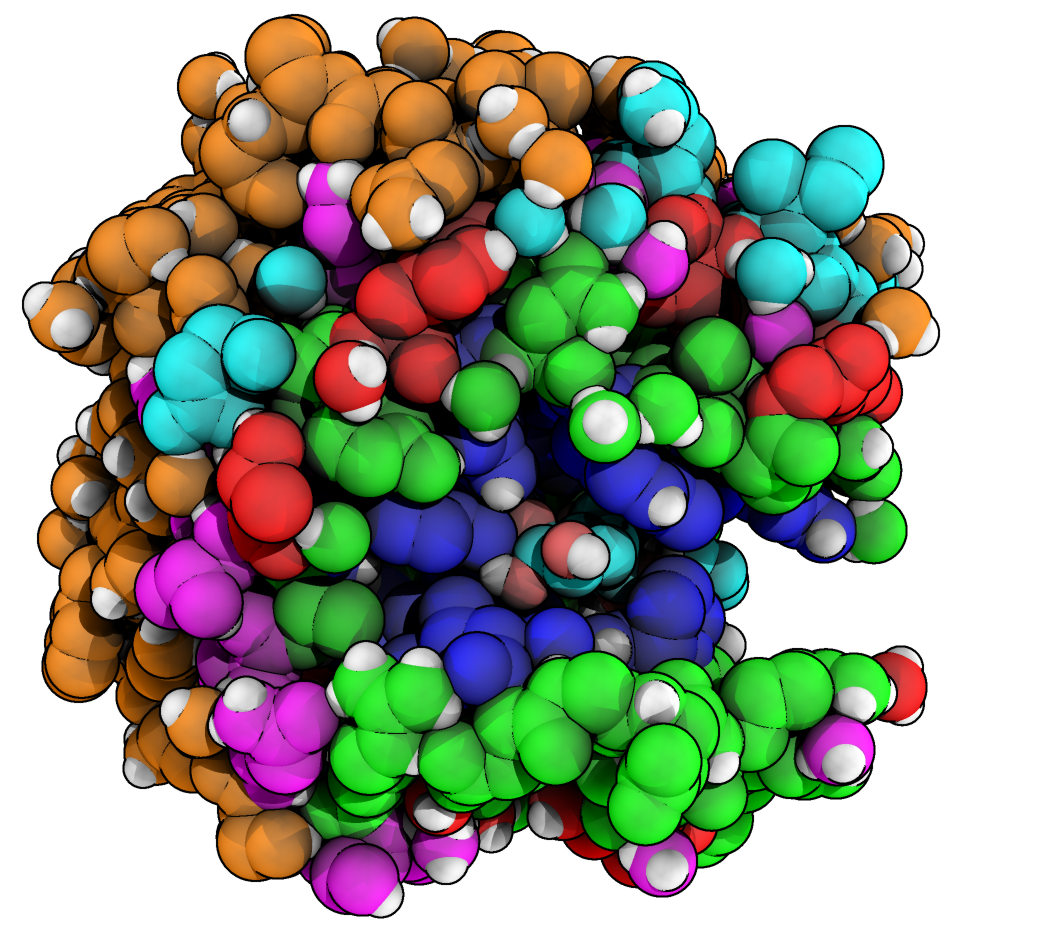
\includegraphics[width=0.95\linewidth]{bcx-constraint-layers-ray-occlusion-2.png}
\end{minipage}
\begin{minipage}{0.51\linewidth}
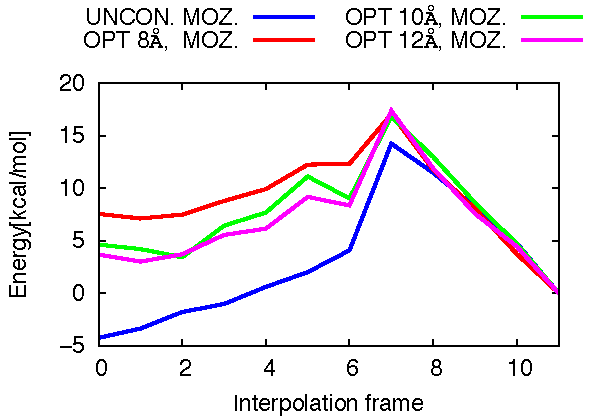
\includegraphics[width=1.00\linewidth]{bcx-barriers-constraint-layers.pdf}
\end{minipage}
\caption{
\textbf{A}: Illustration of optimization layers of BCX with bound ONP substrate.
Color coded residue layers have at least one atom within the indicated distance to any atom of the substrate:
\textit{green} 8 \AA, \textit{red} 10 \AA, \textit{purple} 12 \AA, \textit{cyan} 14 \AA.
\textit{Brown} residues remain at their optimized GE geometry, \textit{dark blue} are residues which are screened for active mutations.
The substrate is visible in the center of the dark blue residues.
\textbf{B}: Calculated reaction barriers for different layers of optimized residues (based on Hediger \textit{et al.} (2013b)).
}
\label{fig:bcx_constr_constraint_layers}
\end{figure}
Based on this second approach, \textit{i.e.} using the optimized GE structure as the template for the ES structure, and when not applying any constraints (apart from the reaction coordinate $x_1$), the reaction barrier is found to be 18.5 kcal/mol which is in very close agreement to the experimentally reported value of 17.0 kcal/mol obtained from transition state theory\cite{joshi2000hydrogen}.
This strongly supports that the outlined modeling procedure, the configuration of the quantum chemical method and the included/omitted physical effects provide a meaningful model of the enzyme kinetics.
As pointed out above, when applying constraints on remote parts of the structure, this can decrease the reaction barrier because the ES structure is increased in energy relative to the GE reference point (which is set to zero).
However, it is reasonable to assume that this relative increase will be the same for all studied structures and so cancels out once mutants are compared relative to each other.  
Overall, application of constraints to remote parts of the enzyme is necessary to reach the desired calculation efficiency of one reaction barrier per day when running each interpolation step in parallel.
Furthermore, application of constraints has been widely adopted by the community\cite{himo2006quantum,siegbahn2009recent,liao2012comparison,lonsdale2013quantum}.
The time required for optimizing the structures with or without constraints are found to differ by a factor of six (Fig. 4B in Hediger \textit{et al.} (2013b)).\\
\textbf{Mutant activity screening.}
By a similar approach as the one outline for the modeling of the WT reaction, it is found that different ways of modeling the set of mutants results in significantly different levels of efficiency, both in terms of required manual efforts as well as in computational time requirements.
We refer to the original publication for details\cite{hediger2013computational} but point out that when, similarly as for the WT, the ES structures of the mutants are based on templates of optimized mutant GE structures, again large gains in computational efficiency are possible (see Fig. 7 in Hediger \textit{et al.} (2013b)).\\
Using PYMOL\cite{PyMOLu}, models of all possible single mutants within a given distance of the substrate are prepared (excluding the catalytically active E78 and E172).\footnote{The PYMOL script used for the preparation of the mutants is available at https://github.com/mzhKU/Enzyme-Screening/blob/master/vsc-bcx.py.}
It is noted that in the current implementation of the presented approach, all mutated side chains are in their default ionization state at physiological pH.
Furthermore, in a number of cases it is not possible to introduce a large side chain in a spatially restricted environment, such cases are discarded.
Lastly, instead of using a side chain rotamer library, each mutated side chain is locally optimized (using an empirical builtin PYMOL function) in the environment of the enzyme before being submitted to the quantum calculation.
This approach allowed to screen a set of 317 single mutants, where on average 29 hours are required to complete the calculations of a full reaction barrier using one CPU for each interpolation point.\footnote{All obtained barriers are provided at http://www.scribd.com/doc/133445214/Supp-Mat-Paper-4.}
From this set of single mutants, for every position $i, j, ...$ in the active site, the mutation resulting in the mutant with the lowest barrier $X_i, Y_j, ...$ is identified.
Then, from this set of single mutants $\{K_l\}$, all possible double mutants $(X_i, Y_j)$ are formed.
Analysis of the reaction barriers of the obtained candidates reveals that the set of double mutants on average has lower activation barriers than the set of single mutants.
Furthermore, the lowest barriers are found among the double mutants.
\begin{figure}[htbp] 
\centering
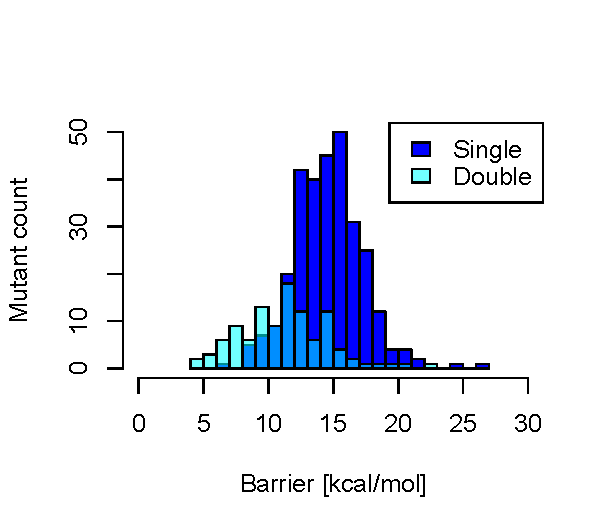
\includegraphics[width=0.95\linewidth]{barrier-distribution.pdf}
\caption{
Barrier distribution of single and double BCX mutants\cite{hediger2013computational}.
The plot is a histogram of reaction barriers, i.e. how many mutants are identified with a given reaction barrier.
}
\label{fig:bcx_barrier_distribution}
\end{figure}
\newline
\textbf{\textcolor{red}{Rationalization of mutants[EXPAND!].}}
Analysis of the set of mutants indicates that position 127 has strong influence on the activity (9 of 20 best single mutants carry a mutation at that position).
Inspection of the structural arrangement of the Q127W, W9D/E and N35E mutations points to a number of possible explanations of the observed lower barriers, Fig. \ref{fig:bcx_rationalization}.
\begin{figure}[htbp] 
\centering
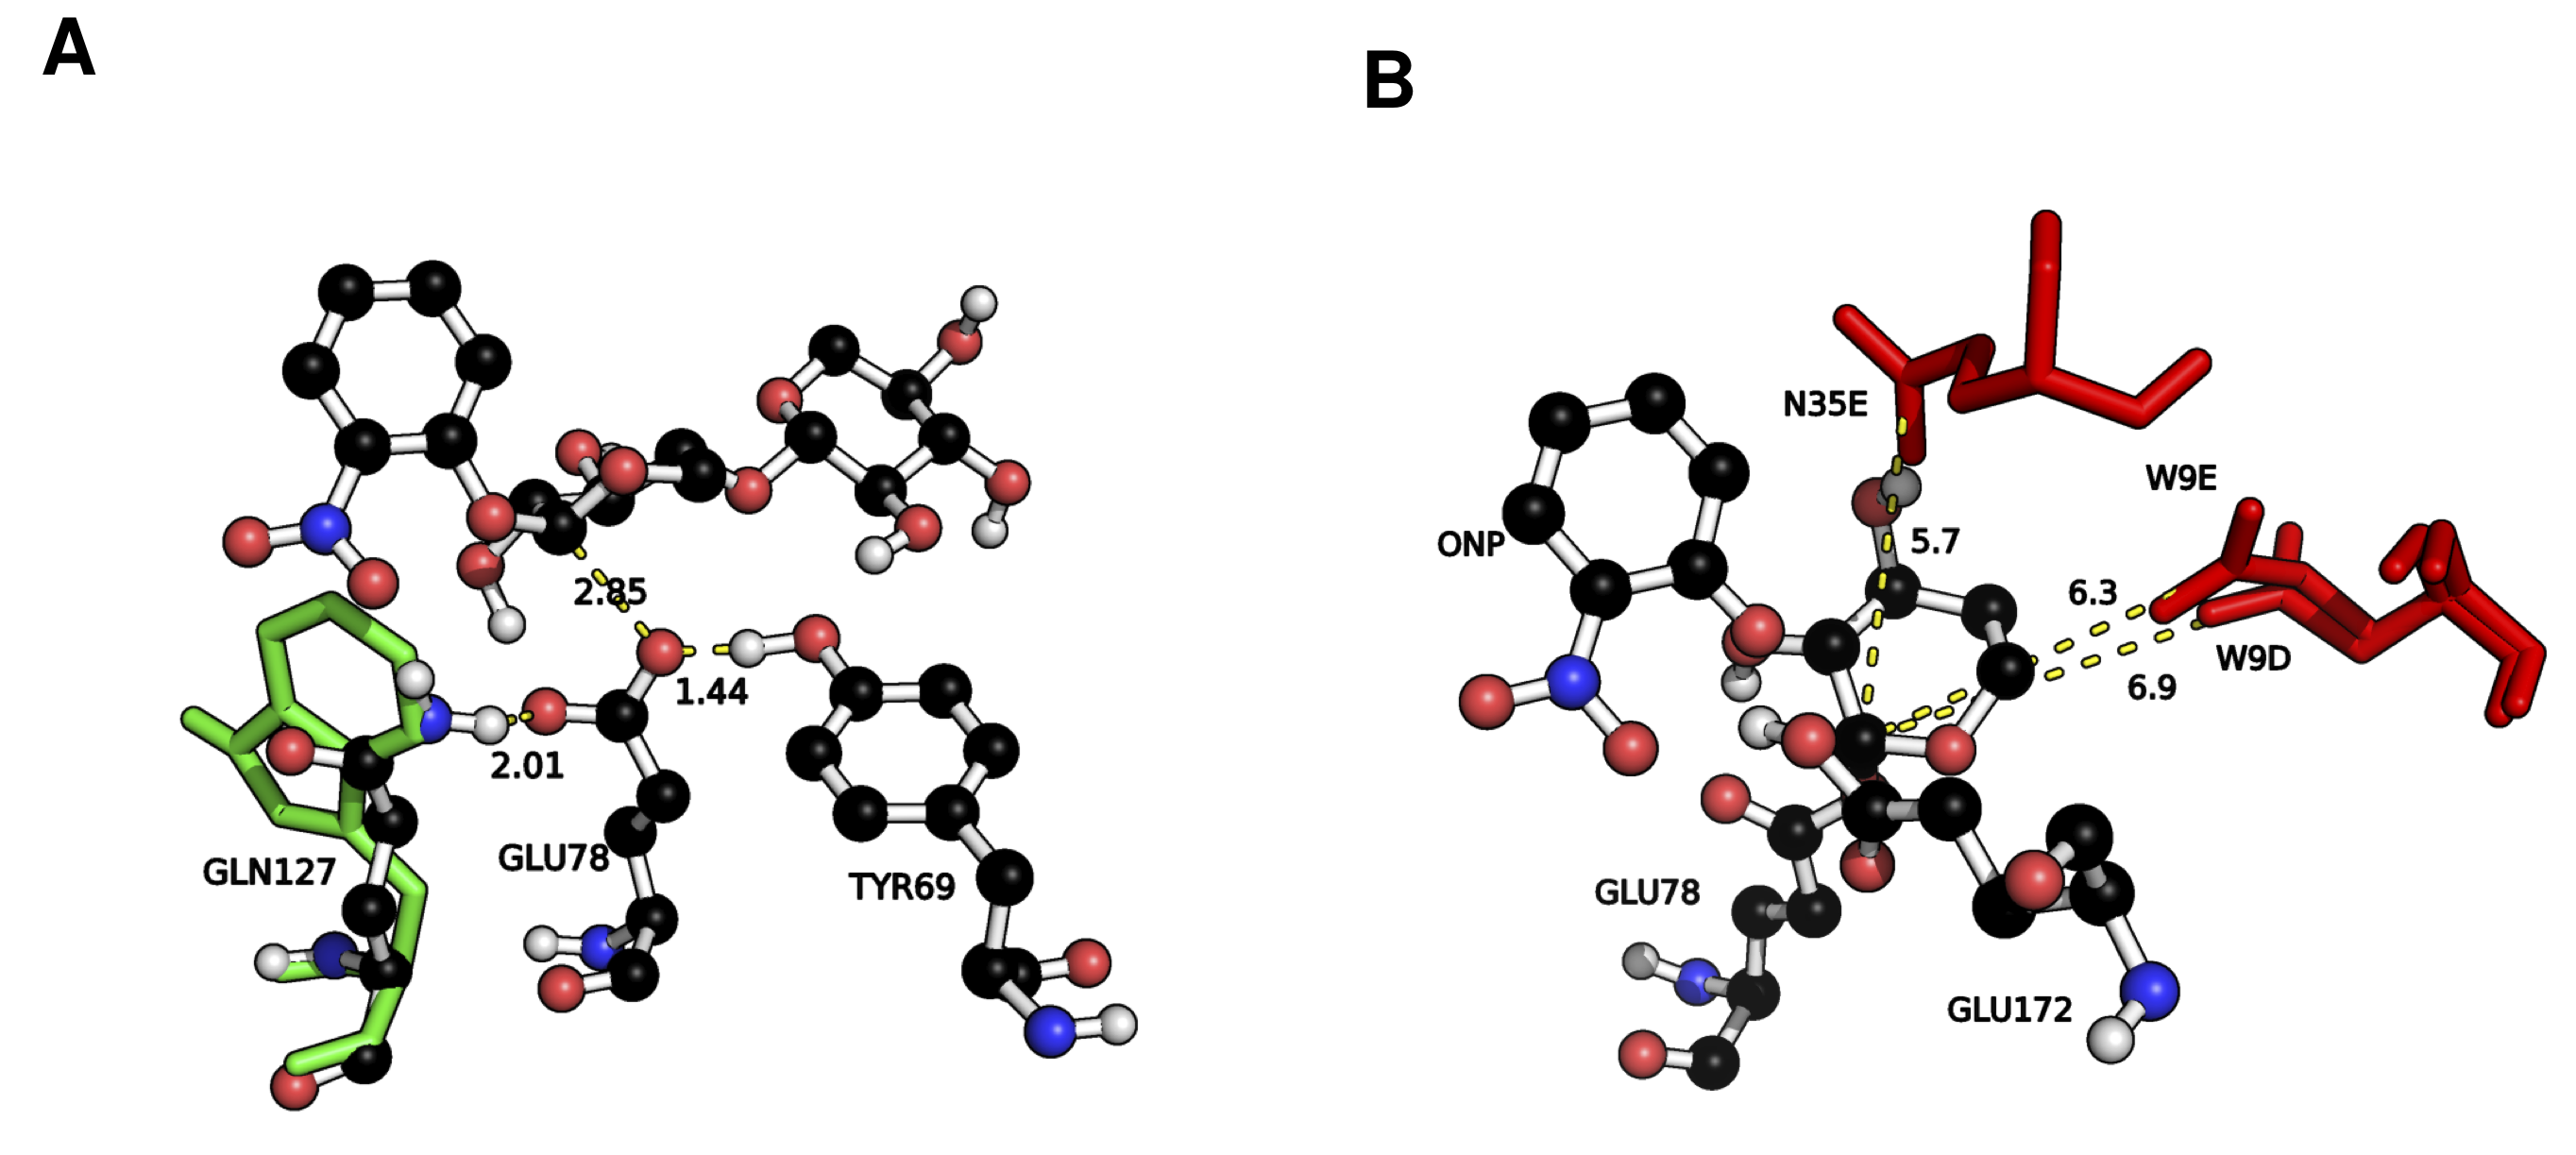
\includegraphics[width=0.99\linewidth]{analyse-charge.png}
\caption{
Rationalization of reaction barriers.
\textbf{A} Overlay of WT (black carbon spheres) and Q127W side-chain (green).
\textbf{B} Stabilizing, coulombic interactions between negative W9D/E or N35E (red) with the nucleophilic, partially positively charged C$_1$ of the substrate.
Distances in \AA\cite{hediger2013computational}.
}
\label{fig:bcx_rationalization}
\end{figure}
As discussed above, the mechanism is postulated to involve a catalytically active, negatively charged E78 residue as the nucleophile.
If Q127 stabilizes the negative charge by hydrogen bonding, the nucleophilic character of E78 is reduced.
Replacing the potential hydrogen bond donor Q127 with a non-hydrogen bonding substitute that can preserve overall structural integrity with a side chain of similar size, such as Q127W, could result in increased nucleophilicity of E78, Fig. \ref{fig:bcx_rationalization} A.
Furthermore, as illustrated in Fig. \ref{fig:bcx_mechanism}, the transition state involves a partially positive charge on C$_1$ of the substrate.
Negative charges on side chains (such as in W9D/E) could act as stabilizers of this negative charge and increase catalytic activity in doing so, \textit{i.e.} by stabilization of the transition state.
Similaryl, when ionized, N35E could act in stabilizing C$_1$ but when in neutral protonation state, it could be acting as a hydrogen bond donor to the catalytically active E172.
This rationalization of N35 mutations would be related to a recently proposed \textit{reverse protonation} mechanism\cite{joshi2000hydrogen}, which still is the subject of ongoing research.\\
\textcolor{red}{[Further discussion of mutants.]}
Contrary to the results from the CALB study, we identified numerous mutants with barriers which are considerably lower than the WT barrier.
This fact might be attributed to significantly promoted catalysis by a better fitting of the substrate in the active site.
%
%\newpage
%\subsection{Further Screening Applications}
%\textbf{The cocaine hydrolase guys}\\
%Make a cocaine hydrolase better\cite{gao2006computational}.\\
%\textbf{Biofuel production}\\
%The bottle neck in biofuel preparation from biobased materials is hydrolysis of cellulosic materials\textcolor{red}{[REFS?]}.
%Development of improved catalysts clearly could boost this field and has immediate impact on company performance.\\
%\textbf{Organic synthesis}\\
%Gotor et al.
% *************************************************************************


% *************************************************************************
% *************************************************************************
\section{Conclusions}\label{sec:conclusions}
The three most significant findings are that firstly, using linear scaling methods and a number of customized software packages it is possible to carry out large scale computational enzyme activity screening studies.
Secondly, single mutant data is not enough to predict combination mutant activities because the activity modulating effects of the point mutations behave non-linearly when in combination with other mutations.
And lastly, using such a screening approach allows not only to identify mutants for further characterization by higher level methods or experimental verification, but also to formulate hypothesis on how the various mutations actually contribute to increased catalysis.
These findings can then be further exploited in future enzyme engineering efforts.
